\chapter{Related Works}

This chapter presents, in the first section, an overview of the different datasets available online for anomaly detection tasks. Next, different autoencoder-based architectures found in literature are presented.

\section{Available datasets}
One of the main reasons for the success of ML or DL algorithms in last years is the availability of more and more public standard datasets, regarded as common benchmarks and that consequently allow a fair comparison between different proposals in literature. In PdM and in anomaly detection tasks, this is not totally true because often machinery data are confidential and sometimes studies are conducted by companies' internal divisions and the consequence is that observations are not made available publicly. In response to this need, in the last years some datasets have been built and then made available online (Table \ref{datasets-table}).\\

% Please add the following required packages to your document preamble:
% \usepackage{booktabs}
\begin{table}[ht]
\small
\centering
\begin{tabularx}{\textwidth}{cl}
\hline
Dataset Name & Summary \\ \hline
CWRU & \begin{tabular}[c]{@{}l@{}}Ball bearing test data for normal and faulty bearings. \\ Motor bearings were seeded with faults using electro-discharge\\ machining (EDM) and vibration data was collected using \\ accelerometers, which were attached to the housing \\ with magnetic bases.\end{tabular} \\ \hline
MFPT & \begin{tabular}[c]{@{}l@{}}Provides time-series data from nominal, outer race fault at \\ various loads, inner race fault at various loads and three\\ real-world faults of bearings\end{tabular} \\ \hline
NAB & \begin{tabular}[c]{@{}l@{}}Contains cross-domain data collections, like \\ the average CPU usage in AWS cluster or the internal \\ temperature data of an industrial machine.\end{tabular} \\ \hline
Yahoo S5 & \begin{tabular}[c]{@{}l@{}}Consists of four data classes, each of which contains either a\\  set of synthetic or real web traffic metrics tagged with anomalies\end{tabular} \\ \hline
DCASE2020 & \begin{tabular}[c]{@{}l@{}}The dataset consists in sounds collected \\ from different industrial machines. It is composed by MIMII \\ Dataset and ToyADMOS.\end{tabular} \\ \hline
\end{tabularx}
\caption{Anomaly detection online available datasets.}
\label{datasets-table}
\end{table}

To clarify, these datasets contain some anomalous observations generated manually by operators, but, as mentioned in the first chapter, they not represents all the possible anomalous states and they are only used to build test set and consequently evaluate the performance of the models, trained in unsupervised way with the use of only normal states data. 

\section{Anomaly detection with autoencoders}
In this section, some autoencoder-based architectures found in literature are presented.
Antonio L. Alfeo et al. \cite{12UsingAEinManufacturing} show an autoencoder-based approach with different case studies addressing industrial laundry assets’power consumption and bearing vibrations. In the first case, the time-series data are realistically created using the official information of assets’ manufacturers (e.g. nominal energy consumption) and the details provided by researchers' industrial partner. In the second case, time-series are extracted from MFPT dataset presented in Table \ref{datasets-table}. After the creation of these ad-hoc datasets, the proposed approach employs an autoencoder to score the anomaly degree of each input instance (presented as rescaled time-series features), after it has been trained with regular occurrences. The reconstruction errors, calculated downstream of the decoder, are further processed by the discriminator, which rescales them between 0 and 1 by using a sigmoidal function (Figure \ref{autoencoder_plus_discriminator}).
\begin{figure}[ht]
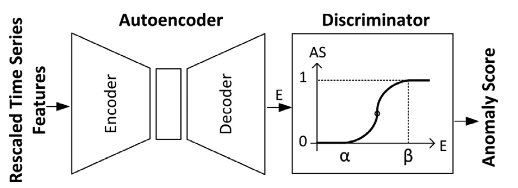
\includegraphics[scale=0.7]{TESI DI FIORE/img/Autoencoderplusdiscriminator.png}
\centering
\caption{Anomaly detector architecture proposed by \cite{12UsingAEinManufacturing}.}
\label{autoencoder_plus_discriminator}
\end{figure}
For both the dataset, the inputs of the architecture are samples characterized by statistical features extracted from time-series available in the dataset which capture their trends of them over time (like 90th, 75th, 50th and 25th percentile of the time series or the mean absolute deviation).\\
Ruei-Jie Hsieh et al \cite{9UnsupervisedOnlineAnomalyDetectionMultivariate} developed an unsupervised deep RNN (Recurrent Neural Network) detection model based on the LSTM (Long Short Term Memory) autoencoder. The recurrent layers of the autoencoder allow to capture temporal dependencies in multivariate sensor data provided by a manufacturing company. The mentioned company has a production line in which there are three chambers (A,B,C) disposed in series and the product moves from a chamber to another. Each chamber has 4 sensors (W,X,Y,Z) for the detection of the products passage. When sensors outputs signal 1, it indicates the product is already in a chamber, otherwise it outputs 0. Obviously, the anomalies in data are not detectable in the single values generate by sensors, but only in the time sequence of them. This is the reason of using LSTM cells to build encoder and decoder layers. The detection of an anomalous behaviour in a chamber prevents that the products pass in the whole production line (early detection). Autoencoder models are trained to reconstruct input sequences, timestamp by timestamp, using a sliding-window method (sequence-to-sequence autoencoder). The input vector in each timestamp is composed by the outputs of the four sensors in a chamber. Using a threshold $\epsilon$, defined using the reconstruction error of training data, each timestamp of each sequence is labeled as normal or anomalous on the basis of its reconstruction error. In conclusion, as each timestamp is labeled as many time as the sliding window length, a majority voting mechanism is applied to make the final decisions and eventually an alert is generated (Figure \ref{seq2seq-architecture}).
\begin{figure}[ht]
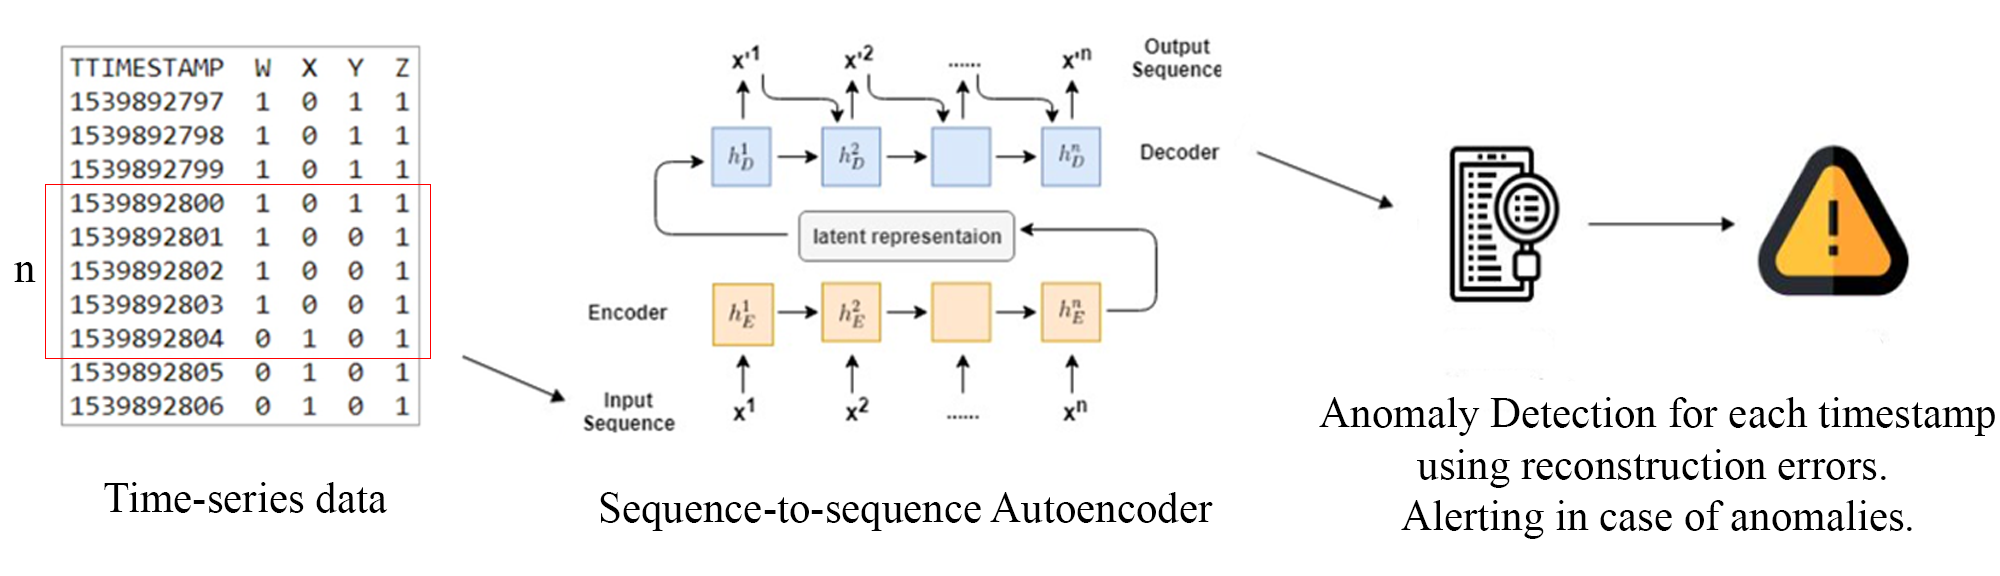
\includegraphics[scale=0.9]{TESI DI FIORE/img/sequence-to-sequecen-ae-anomalydetection.png}
\centering
\caption{Architecture pipeline proposed by \cite{9UnsupervisedOnlineAnomalyDetectionMultivariate}.}
\label{seq2seq-architecture}
\end{figure}\\
Another strategy to resolve the anomaly detection task is to combine deep learning and ensemble learning. Shao Haidong et al. \cite{14NovelMethodEnsembleDeepAutoencoder} propose a novel method called ensemble deep autoencoders (EDAEs) for the intelligent fault diagnosis of bearings, using CWRU dataset. The ensemble of multiple deep autoencoders is a good choice to overcome the low generalization ability of individual deep autoencoders. Diversification is obtained by designing deep autoencoders with different kind of activation functions, because neural networks differing in activation functions usually show different characteristics and complementary learning behaviours. As combination strategy, the authors define a new one. For each deep autoencoder the classification accuracy is calculated and then compared to a pre-defined threshold. Only autoencoders with accuracy greater than the threshold are kept. Using accuracies, different weights are calculated and then assigned to each model and at the end, the achitecture reports the combined diagnosis result of each sample based on the weight scores. In order to maintain the stability of the combined diagnosis results, repeated trials are carried out. The results (in terms of precision, recall and F-Measure), shown in the paper, demonstrate the validity of this architecture.\\
The existing anomaly detection systems used in the industrial domain depend on the properties of sensors. Among those systems, most common are visual anomaly detection systems, which have some drawbacks such as illumination, occlusion by objects, being out of the field of view, and so forth, which strongly affect the performance of the system, also in terms of computation power needed to achieve real time performance. The Anomalous Sound Detection (ASD) systems, however, are not affected by the problems just described, and thus offer an advantage using acoustic data features, especially in terms of computation power needed for real time detection and of simplicity in collecting data. A drawback of using acoustic data is that they must be transformed to be compatible with the training processes of autoencoder models. In fact, compared to images, audio clips need some pre-processing steps in order to convert them in different formats compatible with neural network training process, like signals composed by air pressure values or spectrograms, often in the Mel scale\footnote{Mel spectrograms derive from a particular cepstral representation of the audio signal. The difference between the cepstral and the mel-frequency cepstral representation is that, in the MFC one, the frequency bands are equally spaced on the Mel scale, which approximates the human auditory system’s response more closely than the linearly-spaced frequency bands used in the normal cepstral transformation.}.\\
In this context, the authors of \cite{13RealTimeDetectionUsingSequentialAutoencoder} compare the performances of convolutional LSTM autoencoder (Conv-LSTMAE)  and sequential convolutional autoencoder (CAE) using sounds retrieved from Youtube videos recorded during industrial manufacturing processes. Because it is hard to capture abnormal patterns due to their rarity in real life and because the creation of anomaly events and recording respective sounds is expensive, the authors generate artificially anomalous samples for testing adding anomaly events like explosion, fire or glass breaking to downloaded clips. Although the proposed two autoencoders are different in terms of layers, the pipeline of the system is fixed: there are sequences of five 128x128 spectrograms (extracted from audio dataset) that are the inputs of sequence-to-sequence encoding and decoding networks, which generate output sequences that must be as much as similar to the input ones. Also this time, the decision about the generation of an alert due to the possible presence of anomalies, is made on the comparison between the reconstruction error of each spectrogram to a pre-defined threshold.

\section{Anomalous sound detection with DCASE dataset}
Detection and Classification of Acoustic Scenes and Events, is a community that organizes challenges every year and usually their task 2 regards machineries sound data. The dataset presented in the Table \ref{datasets-table} is provided by DCASE 2020 Challenge, which title is "\textit{unsupervised detection of anomalous sounds for machine condition monitoring}". Because of only normal working machines sound samples are provided as training data (in form of clips, lasting 10 or 11 seconds), the task must be resolved in unsupervised way, and again autoencoder is one of the best unsupervised approach to do this. In details, the dataset that can be downloaded is composed by ToyADMOS Dataset and MIMII Dataset \cite{DCASE} and refers to different sounds recorded with microphones disposed around different machine types: a Toy-car, a Toy-Conveyor, a valve, a pump, a fan and a slide rail. To make the challenge more interesting, for each machine type different kinds of machines are considered, identified by a numeric ID (for example different kinds of pump). A baseline system implementation for comparison purpose was made available by the authors of the challenge. It consists of a dense autoencoder with three layers, in both the encoder and decoder components, with 128 units, and a latent space with 8 units, all with the ReLU activation function. Following, a summary of most interesting approaches to improve the baseline system is shown, while, in the next chapters, the dataset is explored more in details to support a better explaination of the experimental part of this work.\\
% LITERATURE
Pilastri et al. \cite{15DeepDenseConvAE} propose two deep learning models, based on a dense and convolutional architectures fed with Mel spectrograms. For the dense one, the encoder and decoder networsks consist of four fully-connected layers, followed by Batch Normalization and ReLU as the activation function. For the convolutional one, the encoder and decoder networks are comprised of convolutional layers with Batch Normalization and the ReLU activation function after each convolution. In both architectures the goal is to minimize the reconstruction error between inputs and outputs. Regarding features extraction, for the dense autoencoder, audio samples are buffered in fixed-length 1 second intervals with a 50\% overlap and, after the extraction of Mel spectrograms 128x640 dimensional input matrix are obtained. In the convolutional autoencoder system, the mel spectrograms obtained from samples are segmented to form 128x32 frames, ready for training. As for previous described architectures, the classification of audio clips, is made comparing the reconstruction error (in terms of mse) and a pre-defined threshold. Results show that for two machine types (slider and valve), the best results were achieved by the convolutional autoencoder, while the dense autoencoder provided the best results for the others.\\
Again, also in anomalous sound detection task, some LSTM-based autoencoders architecture can be found in literature. For example, in the technical report provided by Jalali et al. \cite{16LSTMDeepAutoencodersForASDtask}, the architecture encodes the information using LSTM layers with \textit{n} units and then their outputs are passed into a bottleneck layer, which is also a LSTM layer with smaller size together with a repeat vector layer. A repeat vector layer repeats its input vector multiple times (the number of time steps chosen for the sequences). Next, a stack of sequential LSTM layers reconstruct the original input.\\
Another interesting approach is the one proposed by Tomoki Hayashi et al. \cite{17ConformerBasedIDAWAREAutoencoder}. Their paper presents a Transformer-based and Conformer-based autoencoder for ASD, performing sequence-by-sequence processing. As opposed to the standard autoencoder, this kind of architectures can extract sequence-level information from whole audio inputs, using a methodology called self-attention mechanism, with whom Trasformer and Conformer neural networks are built. In fact, a critical disadvantage classic sequence-to-sequence autoencoder is the inability of the system to retain longer sequences. The attention mechanism was created to resolve this problem of long dependencies, as it is an interface connecting the encoder and decoder providing to the decoder the information from every encoder hidden state. With this framework, the model is able to selectively focus on valuable parts of the input sequence and hence, learn the association between them.\\
As can be noted, all the approaches proposed above differ from the way autoencoders are built. In fact, the main idea is always to train autoencoders to reconstruct as well as possible the normal audio samples provided in input and then to detect anomalies when there is some input that are badly reconstructed by the architecture. In literature, however, there are also some proposals that are regardless of how the autoencoders are build. For example, the authors of \cite{18IDConditionedAutoEncoder}\cite{19DescriptionDiscussionDCASE2020} and also the same researchers of the last presented approach, introduce the concepts of ID conditioning and ID regression. The main idea of both is to use the information related to the particular device identifier from which the input sound clips is retrieved to influence the autoencoder behaviour. In case of ID embedding, the machine ID (which identifies the brand of the particular machine type) is concatenated or added to the latent variables extracted by the encoder. This makes possible to inform the decoder of the machine ID information explicitly, allowing the training of only one model for the all the available machine brands. In the case of the ID regression, the idea is to concatenate the machine ID to the input features, and the autoencoder then reconstructs not only the input acoustic features but also the machine ID. The reason of this is that the autoencoder tends to confuse the machine ID when the audio clip includes an anomalous sound even if the correct machine ID is provided as the inputs. Therefore, the model can detect whether the audio clip includes an anomalous sound from the estimated machine ID.